\documentclass[../../main.tex]{subfiles}

\begin{document}

\section{Puente de Wien}

\subsection{Diseño del puente}
\begin{figure}[H]	
	\centering
	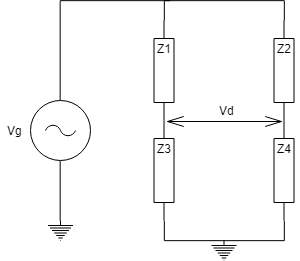
\includegraphics[width=0.35\textwidth]{fotos/PuenteGen.png}
	\caption{Puente con Impedancias genericas} \label{fig:pg}
\end{figure}
La tensión de salida del puente de la figura \ref{fig:pg}, es $V_d=V_g \frac{Z_3 Z_2 - Z_1 Z_4}{(Z_1 + Z_3)(Z_2 + Z_4)}$. En el equilibrio ($V_d=0$), se cumple que $Z_1 Z_4 = Z_2 Z_3$. En el caso del puente de Wien $Z_1=R_1 + \frac{1}{SC_1}$, $Z_2=R_2$, $Z_3=R_3 +  \frac{1}{SC_3}$ y $Z_4=R_4$. En el equilibrio se cumple que $\frac{C_3}{C_1} \frac{R_1}{R_3}= \frac {R_2}{R_4}$ y $f=\frac{1}{2 \pi \sqrt{R_1 R_3 C_1 C_3} }$. Si $R=R_1=R_3$, $C=C_1=C_3$ y $R_2=2 R_4$ entonces $f=\frac{1}{2 \pi RC}$.

\subsubsection{Elección de componentes}
Asumiendo que  $R=R_1=R_3$ ,$C=C_1=C_3$ y $R_2=2 R_4$ , se obtuvo que  $f=\frac{1}{2 \pi RC}$. El intervalo de frecuencias que se desea medir es $f \in [10KHZ , 100KHz]$, fijando $C=820pF$, $R_2=20K\Omega$ y $R_4=10K\Omega$  entonces $R \in \left[ \frac{1}{2 \pi f_{max} C} , \frac{1}{2 \pi f_{min} C} \right]=\left[ 1941 \Omega , 19409 \Omega \right]$. Para conseguir dichos valores de R se utilizó un preset de $25K\Omega $.

\subsubsection{Analizis de sensibilidad}
Tal como ya fue mencionado, $R=R_1=R_3$y dichas resistencias se implementaron con una ressitencia de $1.5K\Omega$ en serie con un preset de $25K\Omega$. El present es de 25 vueltas y suponiendo que lo minimo que se puede girar es un cuarto de vuelta, definimos nuestro $\Delta R=250\Omega$. A ademas se supuso que la maxima diferencia entre una resistencia de ajuste era $\Delta R=250\Omega$, de esta manera se graficaron las sensivilides de $V_d$ respecto de $R_1$ y $R_3$ variando $R$ en el rango indicado en la seccion anterior. Ademas se analizó la sensivilidad de $V_d$ respecto a las mismas resistencias, pero variando la frecuencia en el rango de medición del puente.

\begin{figure}[H]	
	\centering
	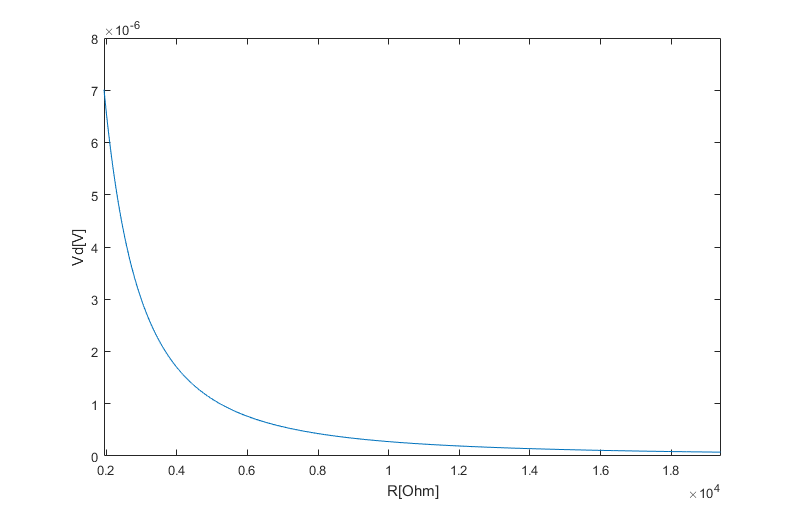
\includegraphics[width=0.7\textwidth]{fotos/r3r.png}
	\caption{Sensivilidad de $V_d$ respecto a R3}
\end{figure}

\begin{figure}[H]	
	\centering
	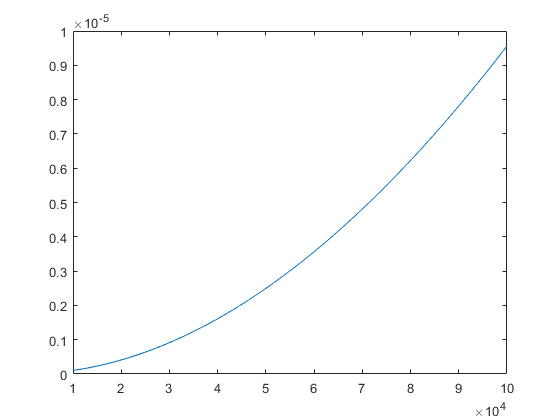
\includegraphics[width=0.7\textwidth]{fotos/r3f.png}
	\caption{Sensivilidad de $V_d$ respecto a R3 variando f}
\end{figure}


\begin{figure}[H]	
	\centering
	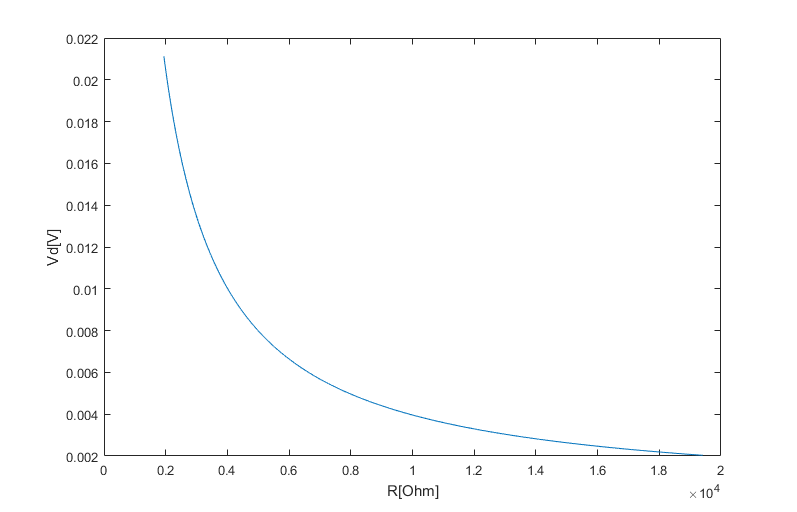
\includegraphics[width=0.7\textwidth]{fotos/r1r.png}
	\caption{Sensivilidad de $V_d$ respecto a R1}
\end{figure}

\begin{figure}[H]	
	\centering
	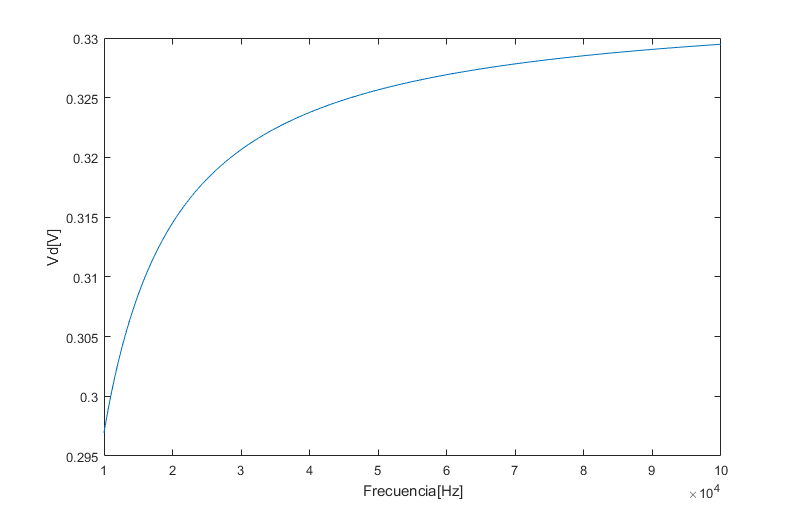
\includegraphics[width=0.7\textwidth]{fotos/r1f.png}
	\caption{Sensivilidad de $V_d$ respecto a R1 variando f}
\end{figure}


Tal como se observa en ambas imagenes la sensibiliada de $V_d$ respecto a ambas resistencias es paracticamnete la misma, por ende una resistencia no enmascara a la otra. Ademas la sensivilidad de ambas resistencias empeora al aumentar la frecuencia.




\subsubsection{Mediciones}
Se midieron las siguientes frecuencias:

\begin{table}[H]
\begin{center}
\begin{tabular}{|l|l|l|l|l|}
\hline
Frecuencia generador$[KHz]$& $R_1 [K\Omega]$ & $R_3[K\Omega]$ & Frecuencia calculada $[KHz]$ &Error[ \% ]\\
\hline \hline
9.7 & 19.4& 19.4&10&3.1  \\ \hline
28.4 & 6.5& 6.5&29.8&5.1  \\ \hline
37.7 & 4.85& 4.85&40&6.1  \\ \hline
54.6 & 3.34& 3.34&58.1&6.4  \\ \hline
75.5 & 2.76& 2.76&70&6.8  \\ \hline
106.5 & 1.94& 1.94&99&8.7  \\ \hline

\end{tabular}
\caption{Mediciones de frecuencias.} 
\end{center}
\end{table}

\subsubsection{Convergencia del puente}
Para analizar la convergencia del puente, se realizó un grafico de $V_d(R,f)$ en matlab variando R y f en los intervalos correspondientes.

\begin{figure}[H]	
	\centering
	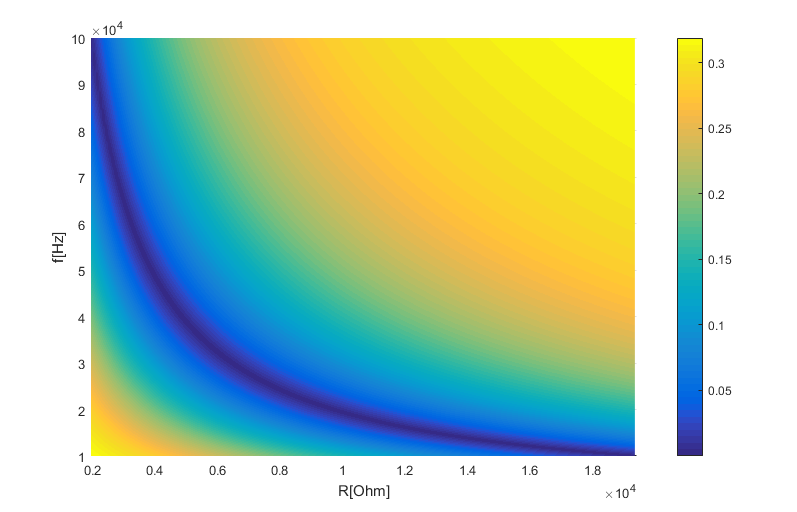
\includegraphics[width=0.9\textwidth]{fotos/conv.png}
	\caption{Grafico $V_d(R,f)$}\label{fig:convw}
\end{figure}

Como se observa en la figura \ref{fig:convw}, hay una unica franja violeta (minimo), esto quiere desir, que existe un unico valor de R para cada frecuencia f que genera un minimo de $V_d$.

\subsubsection{Conclusión}
Como la convergencia del puente es unica para cada vlor de resistencia el puente no necesita un manual para su utilizacion. En cuanto al error que obtuvimos en la medicion lo atrivuimos a que la medicion se realizón con el osiloscopio y sin amplificador de instrumentacion, ademas de a las tolerancias del 10 \% en los capacitores, ademas al hecho que al aumentar la frecuencia aumenta la sensivilidad frente a las variables de ajuste, dicho fenomeno se observa en el hecho de que el error aumenta con el aumento de la frecuencia.

\end{document}

